%%%%%%%%%%%%%%%%%%%%%%%%%%%%%%%%%%%%%%%%%%%%%%%%% PREAMBLE %%%%%%%%%%%%%%%%%%%%%%%%%%%%%%%%%%%%%%%%%%%%%%%%%%

%environment setup
\documentclass[letterpaper,11pt]{article}
\usepackage[square,comma,numbers,sort&compress]{natbib}
\bibliographystyle{ieeetr}
\usepackage{amsmath}
\usepackage{graphicx}
\usepackage{url}
\usepackage{xspace}
\usepackage[left=20mm,top=20mm]{geometry}
\usepackage{hyperref}
\usepackage{lineno}
\renewcommand{\familydefault}{\sfdefault}

%macros
\newcommand{\reffig}[1]{Figure~\ref{#1}}
\newcommand{\refsec}[1]{Section~\ref{#1}}
\newcommand{\refeq}[1]{Equation~\ref{#1}}

%%%%%%%%%%%%%%%%%%%%%%%%%%%%%%%%%%%%%%%%%%%% TITLE AND ABSTRACT %%%%%%%%%%%%%%%%%%%%%%%%%%%%%%%%%%%%%%%%%%%%%

%title
\title{Correcting Image Illumination for Differences in Exposure Time}
\author{Maggie Eminizer\\ \url{margaret.eminizer@gmail.com}\\ JHU Astropath Group}
\date{\today}
\begin{document}
\maketitle

%start numbering lines
\linenumbers

%abstract
\abstract{}

%%%%%%%%%%%%%%%%%%%%%%%%%%%%%%%%%%%%%%%%%%% INTRODUCTION SECTION %%%%%%%%%%%%%%%%%%%%%%%%%%%%%%%%%%%%%%%%%%%%
\section{Introduction}
\label{sec:introduction}

An important step in preparing a protocol for scanning a set of fluorescent tissue sample slides using the Akoya Biosciences Vectra 3.0 or Vectra Polaris digital microscopy systems is specifying the amount of time for which the sample should be exposed to the camera \cite{vectra_user_manual,polaris_user_manual}. The exposure times specified in the protocol are chosen by referencing one or more example tissue regions and making sure the resulting images are sufficiently exposed to show structures of interest yet not saturated so that important details become washed out. One exposure time value is chosen per filter cube, each of which corresponds to several layers of the multiplexed images.

The microscopes also include a software feature called ``saturation protection,'' recommended to be included in every scanning protocol, that automatically adjusts the exposure time of individual high-power fields (HPFs) to prevent them being overexposed due to a greater-than-expected amount of fluorescence, bright dust on the slide, or any other reason \cite{vectra_user_manual,polaris_user_manual}. Therefore, while a scanning protocol does specify a \textit{maximum} exposure time for each broadband filter region, that maximum time is not reached in every case, and the actual exposure times of each image layer group can vary independently between HPFs on the same slide (or between slides). 

An example of exposure time variation is shown in \reffig{fig:exposure_time_variation_M9_1} for different layers of HPFs in the sample called \texttt{M9\_1}. The exposure times for image layers corresponding to the DAPI and Texas Red filter groups are different for many images in the sample, while the layers corresponding to the Cy5 filter group were all exposed for the same amount of time. The variations for layers of this sample in particular are very visible, though not entirely atypical.

\begin{figure}[!ht]
\centering
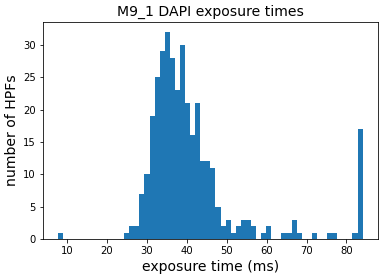
\includegraphics[width=0.3\textwidth]{images/introduction/exposure_times_M9_1_layer_1}
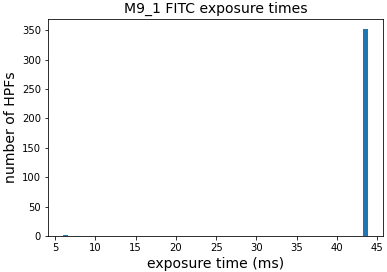
\includegraphics[width=0.3\textwidth]{images/introduction/exposure_times_M9_1_layer_10}
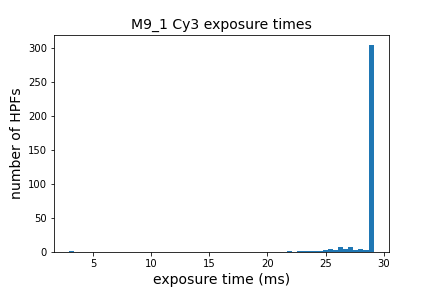
\includegraphics[width=0.3\textwidth]{images/introduction/exposure_times_M9_1_layer_19}
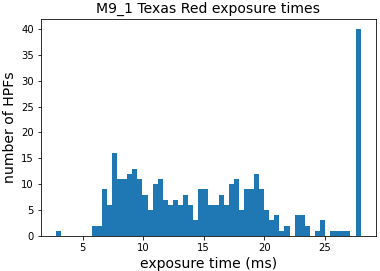
\includegraphics[width=0.3\textwidth]{images/introduction/exposure_times_M9_1_layer_26}
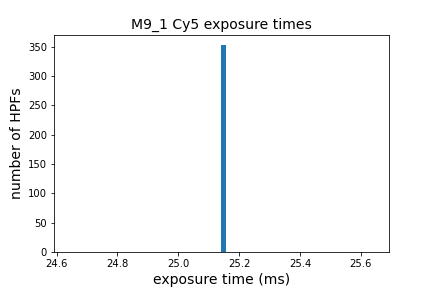
\includegraphics[width=0.3\textwidth]{images/introduction/exposure_times_M9_1_layer_33}
\caption{\footnotesize Exposure times for different layers of HPFs in the dataset ``M9\_1.'' Shown from top left to bottom right are layers 1, 10, 19, 26, and 33, respectively, corresponding to the first layers in each of the DAPI, FITC, Cy3, Texas Red, and Cy5 filter groups, respectively. The DAPI and Texas Red layers show substantial variation in exposure time, while the FITC and Cy3 layers show less variation for this sample, and the Cy5 layers of every HPF were all recorded with the same exposure time.}
\label{fig:exposure_time_variation_M9_1}
\end{figure}

Two example image layers corresponding to those with the minimum and maximum exposure times in the FITC filter group for this sample are shown in \reffig{fig:max_min_M9_1_images} to illustrate the behavior of the saturation protection feature. The minimally-exposed image layer clearly shows the single bright spot that triggered the saturation protection, stopping exposure of that HPF layer before it could be completely washed out by the noise from the spot. The maximally-exposed image layer shows no such localized brightness, and so it was exposed for the full, maximum time specified in the protocol.

\begin{figure}[!ht]
\centering
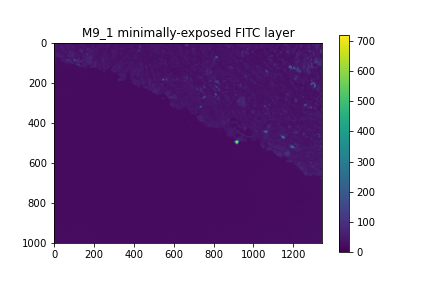
\includegraphics[width=0.45\textwidth]{images/introduction/min_exposure_M9_1_image}
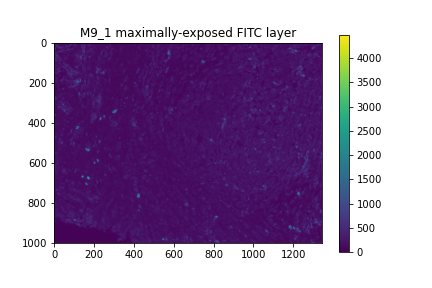
\includegraphics[width=0.45\textwidth]{images/introduction/max_exposure_M9_1_image}
\caption{\footnotesize Layer 11 (corresponding to the FITC filter group) of images in the dataset ``M9\_1'' with the minimum (left) and maximum (right) recorded exposure time. The image layer with the minimum exposure time shows a clear bright spot that triggered the saturation protection feature in the Vectra 3.0 microscope software.}
\label{fig:max_min_M9_1_images}
\end{figure}

But comparing the actual numbers of counts in these image layers shows a challenge that arises from curtailing the exposure of some HPF layers. In the HPF whose FITC layers were exposed for the full, maximum time of 43.8 ms, the fluorescent tissue regions often register over a thousand counts, but the fluorescent tissue visible in the HPF layer exposed for the minimum time of 6.0 ms rarely registers more than a couple hundred counts. While a visual comparison is easily made for a human observer who can recognize that the minimally-exposed image layer shows some dark background, some tissue, and a bright spot, a quantitative comparison of the image counts themselves would not necessarily lead to the same conclusion. When an even greater degree of variation is observed, for example in the DAPI layers of the \texttt{M9\_1} sample, the result is a large number of images whose numbers of counts do not directly translate to the brightness of the fluorescent tissue at each location within the sample.

Differences in exposure time can be simply compensated for by considering counts per unit time rather than total counts, and the inForm and Phenochart softwares both offer ``normalized for exposure'' analysis modes that do exactly that \cite{inform_user_manual,phenochart_user_manual}. While this simple correction may be effective for qualitative or visual analysis of images, it is not sufficient for highly automated and quantitative analyses that rely on image data being as accurate and consistent as possible across large numbers of independent samples. A more sophisticated model applies corrections that are still linear, in that the number of counts collected increases proportionally to the total exposure time, but with an important offset for a small number of counts, called the ``dark current,'' representing noise in the camera that is present regardless of exposure to fluorescent tissue. 

\refsec{sec:methods} describes the methods developed and the data used to measure the dark current offset as a function of image layer using portions of tissue that are multiply imaged in an overlapping fashion. \refsec{sec:results} details the results of the investigations, and the impact that applying the correction model has to finding layer-dependent thresholds for background illumination. \refsec{sec:summary} gives a brief summary.

%%%%%%%%%%%%%%%%%%%%%%%%%%%%%%%%%%%%%%%%%%%%%% METHODS SECTION %%%%%%%%%%%%%%%%%%%%%%%%%%%%%%%%%%%%%%%%%%%%%%
\section{Methods}
\label{sec:methods}

%%%%%%%%%%%%%%%%%%%%%%%%%%%%%%%%%%%%%%%%%%%%%% RESULTS SECTION %%%%%%%%%%%%%%%%%%%%%%%%%%%%%%%%%%%%%%%%%%%%%%
\section{Results}
\label{sec:results}

%%%%%%%%%%%%%%%%%%%%%%%%%%%%%%%%%%%%%%%%%%%%%% SUMMARY SECTION %%%%%%%%%%%%%%%%%%%%%%%%%%%%%%%%%%%%%%%%%%%%%%
\section{Summary}
\label{sec:summary}

%%%%%%%%%%%%%%%%%%%%%%%%%%%%%%%%%%%%%%%%%%%%%%% BIBLIOGRAPHY %%%%%%%%%%%%%%%%%%%%%%%%%%%%%%%%%%%%%%%%%%%%%%%%
\clearpage
\bibliography{references}

\end{document}